\section{Déroulement du projet}


\subsection{Plannification}

Le projet se décompose essentiellement en trois parties : 

\begin{itemize}
\setlength{\itemindent}{.2in}
\item Bibliographie pour déterminer les programmes à utiliser, et rédaction du cahier des charges
\item Développement et évaluation du pipeline sur un jeu de données de référence
\item Déploiement sur le cloud
\end{itemize} 

Le projet comprendra également, une formation au langage Ocaml, prise en main de la librairie bistro. 
Les différentes tâches seront partagées entre les étudiants. Certaines personnes se concentreront plutôt sur déploiement du pipeline sur le cloud et d’autres sur le développement et le test du pipeline. 



 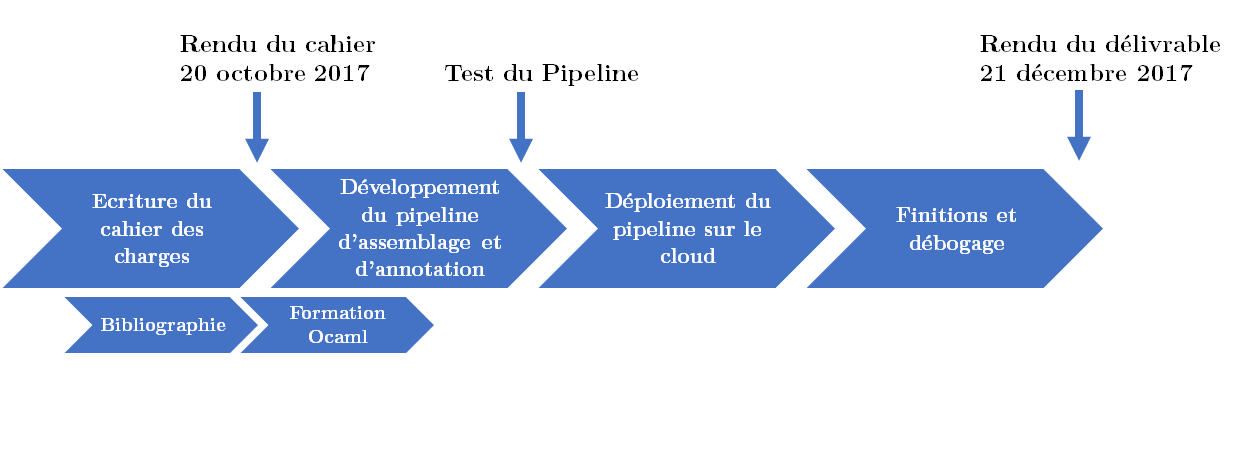
\includegraphics[width=170mm]{images/planning.png}


\subsection{Description des étapes du pipeline et logiciels utilisés}

\subsubsection{Contrôle qualité et trimming des séquences brutes}

\forceindent FASTQScreen : analyse de contamination

\forceindent FASTQC-trimmomatic : contrôle qualité et trimming de lectures courtes

\forceindent LORDEC: contrôle qualité et trimming de lectures courtes 


\subsubsection{Assemblage des lectures}

\forceindent SPAdes \cite{spades}: assembleur conçu pour l'assemblage de novo de génomes bactériens

\forceindent QUAST \cite{gurevich2013quast} : contrôle qualité de l'assemblage (si un génome de référence est disponible)

\subsubsection{Alignement contre génome de référence}

\forceindent BOWTIE2 \cite{langmead2012fast}: aligneur de reads longs contre un génome de référence indexé

\subsubsection{Annotation du génome}

\forceindent ORFinder : détection de gènes de novo

\forceindent BLAST \cite{camacho2009blast+}: annotation comparative et détection de gènes homologues

\forceindent PROKKA : annotation de génomes procaryotes

\subsection{Plan d'assurance qualité}

Pour s’assurer de la qualité du pipeline d’assemblage/annotation, il sera testé sur un jeu de données test de séquençage d’une espèce bactérienne bien annotée dans les bases de données. A priori, les données d’Escherichia coli seront utilisée. Un jeu de données de séquençage Illumina devra être trouvé.


\subsection{Responsabilités}
\textbf{Maîtres d'ouvrage}

Philippe Veber et Stéphane Delmotte (LBBE) sont les maîtres d'ouvrage de ce projet. Les contraintes de temps sont imposées par le Master 2 Bioinformatique de l’université Lyon 1.

\textbf{Maîtres d'oeuvre}

Les quatres étudiants concernés par le projet sont maîtres d’oeuvre, à savoir Lucía Castro García, Cécile Hilpert, Sumaira Javaid et Krystian Valenducq.
